\clearpage

\section{Limits of functions}
Closely related to the idea of continuity is the concept of limits:
\begin{ndef}{: Limit of a function}
	Suppose \(\mc{X},\mc{Y}\) are metric spaces with \(f:\mc{X}\to\mc{Y}\) and \(x_0\in\mc{X}\); we say 
	\begin{equation*}
		\lim_{x\to x_0}f(x_0)=y_0
	\end{equation*}
	exactly when 
	\begin{enumerate}[(i)]
		\item \(x_0\in\mc{X}'\).
		
		\item \(\displaystyle\pfi(x)=\begin{cases}
										f(x)&\text{if}~x\neq x_0\\
										 y_0&\text{if}~x=x_0
									 \end{cases}\) is continuous at \(x_0\).
	\end{enumerate}
	Equivalently,
	\begin{enumerate}[(i)]
		\item \(x_0\in\mc{X}'\).
		
		\item For all \(\eps>0\), there exists \(\delta>0\) such that for all \(x\in\pball{x_0}{\delta}\), \(d_Y(f(x),y_0)<\eps\).
	\end{enumerate}
\end{ndef}
\begin{note}
	For (ii), a sequential alternative exists, namely: \(f(x_n)\to y_0\) for any sequence \(x_n\to x_0\), \(x_n\neq x_0\) for all \(n\).
\end{note}

\begin{figure}[htbp]
	\centering
	\begin{tikzpicture}
		\draw[Latex-Latex, thick] (-3.5,0)--(3.5,0);
		
		\node[below] at (3.5,0) {\(x\)}; 
		
		\draw[Latex-Latex, thick] (0,-2)--(0,3.5);
		
		\node[left] at (0,3.5) {\(y\)}; 
		
		\draw[-, thick, smooth, domain = -3:3, samples = 100, variable = \x, red] plot ({\x}, {sqrt(\x + 3) - 1});
		
		\draw[fill = white!60!white] (2,1.236) circle (1.5pt);
		
		\draw[fill = red!60!white] (2,0.55) circle (1.5pt); 
		
		\draw[-, dashed, red, thick] (-3.5,0.732)--(3.5,0.732);
		
		\node[left, above] at (-0.2,0.732) {\(\color{red} y_0\)};
		
		\draw[-{[scale=0.5]Latex}, thick] (2,1.75)--(2,1.31);
		
		\node[above] at (2,1.7) {\(\varphi\) \small fills this hole};
	\end{tikzpicture}
	\caption{Plot demonstrating the definition above.}
\end{figure}

\clearpage

\section{Differentiation}

\subsection{Basics}
\begin{ndef}{: Differentiability}
	Given an interval \([a,b]\subseteq\R\), a point \(c\in[a,b]\), and \(f:[a,b]\to\R\), let 
	\begin{equation*}
		f'(c)=\lim_{x\to c}\frac{f(x)-f(c)}{x-c}.
	\end{equation*}
	When this limit converges, this is called the ``the derivative of \(f\) at \(c\)". Say ``\(f\) is \emph{\textbf{differentiable}} at \(c\)" when this happens.
\end{ndef}

\begin{figure}[htbp]
	\centering
	\begin{tikzpicture}[scale=1.5]
		\draw[Latex-Latex, thick] (-1,0)--(4.5,0);
		
		\node[below] at (4.5,0) {\(x\)}; 
		
		\draw[Latex-Latex, thick] (0,-1)--(0,3);
		
		\node[left] at (0,3) {\(y\)}; 
		
		\draw[-, thick, smooth, domain = 0.5:4.5, samples = 100, variable = \x] plot ({\x}, {sqrt(\x - 0.5) - 0.5});
		
		\draw[-, thick, smooth, domain = -0.7:4.5, samples = 100, variable = \x, red] plot ({\x}, {0.4*(\x + 1) - 0.6});
		
		\draw[-, dashed, thick] (0.977,0.191)--(0.977,0);
		
		\draw[-, dashed, thick] (3.773,1.309)--(3.773,0);
		
		\node[below] at (0.977,0) {\(c\)};
		
		\node[below] at (3.773,0) {\(x\)};
		
		\draw[fill] (0.977,0.191) circle (1pt);
		
		\draw[fill] (3.773,1.309) circle (1pt);
		
		\node[right, above] at (2,2) {\small slope \(=\displaystyle\frac{f(x)-f(c)}{x-c}\)};
	\end{tikzpicture}
	\caption{Plot demonstrating the definition above.}
\end{figure}

\subsubsection{Instantaneous slope}
When \(f'(c)\) exists, it tells us the slope of the ``best linear approximation" for \(f(x)\) near \(x=c\). Comparing with \(\ell(x)=f(c)+m(x-c)\):

\begin{ntheorem}{: Butterfly lemma}
	In the setup above, 
	\begin{enumerate}[(i)]
		\item If \(m<f'(c)\), then there exists \(\delta>0\) such that 
		\begin{align*}
			&\ell(x)>f(x)\quad\text{for all}~x\in(c-\delta,c)\\
			&\ell(x)<f(x)\quad\text{for all}~x\in(c,c+\delta).
		\end{align*}
		
		\item If \(m>f'(c)\), then there exists \(\delta>0\) such that 
		\begin{align*}
			&\ell(x)<f(x)\quad\text{for all}~x\in(c-\delta,c)\\
			&\ell(x)>f(x)\quad\text{for all}~x\in(c,c+\delta).
		\end{align*}
	\end{enumerate}
\end{ntheorem}

\begin{figure}
	\centering
	\begin{tikzpicture}[scale=1.5]
		\draw[Latex-Latex, thick] (-1,0)--(4.5,0);
		
		\node[below] at (4.5,0) {\(x\)}; 
		
		\draw[Latex-Latex, thick] (0,-1)--(0,3);
		
		\node[left] at (0,3) {\(y\)}; 
		
		\draw[-, thick] (1,-0.2) to [curve through = {(1.96,2)}] (4,2.8);
		
		\draw[thick, dashed, samples = 100, domain = -0.5:4, variable = \x] plot ({\x}, {\x + 0.0426});
		
		\draw[thick, samples = 100, domain = 0.5:3.2, variable = \x, red] plot ({\x}, {2*\x - 1.92});
		
		\draw[thick, samples = 100, domain = -0.5:4.4, variable = \x, blue] plot ({\x}, {0.5*\x + 1.02});
		
		\node[left] at (3.2,4.98) {\(\color{red} f(c)+m(x-c)\)};
		
		\node[left] at (3.2,4.48) {\(\color{red} m>f'(c)\)};
		
		\node[below, right] at (4.3,3.52) {\(\color{blue} \small f(c)+m(x-c)\)};
		
		\node[below, right] at (4.3,3.02) {\(\color{blue} \small m<f'(c)\)};
		
		\draw[-, thick, dashed] (1.96,2)--(1.96,0);
		
		\node[below] at (1.96,0) {\(c\)};
		
		\node[] at (1.46,0) {(};
		
		\node[] at (2.46,0) {)};
		
		\node[below] at (1.46,0) {\(\small c-\delta\)};
		
		\node[below] at (2.46,0) {\(\small c+\delta\)};
	\end{tikzpicture}
	\caption{Visualization of the theorem above.}
\end{figure}

\begin{comment}
	\draw[-, thick, smooth, domain = 0.5:4.5, samples = 100, variable = \x] plot ({\x}, {sqrt(\x - 0.5) - 0.5});
	
	\draw[-, thick, smooth, domain = -0.7:4.5, samples = 100, variable = \x, red] plot ({\x}, {0.3*\x - 0.05916});
	
	\draw[-, thick, smooth, domain = 0.5:2, samples = 100, variable = \x, blue] plot ({\x}, {3*\x - 3});
	
	\node[right] at (2,3.5) {\small \color{blue}\(f(x)+m(x-c)\)};
	
	\node[right] at (2,3) {\small \color{blue}\(m>f'(c)\)};
	
	\draw[-, dashed, thick, smooth, domain = -0.7:4, samples = 100, variable = \x] plot ({\x}, {0.97*\x - 0.788924});
	
	\node[right, below] at (4.5,1) {\small \color{red}\(f(x)+m(x-c)\)};
	
	\node[right, below] at (4.5,0.63) {\small \color{red}\(m<f'(c)\)};
	
	\draw[-, dashed, thick] (1.0892,0.2676)--(1.0892,0);
	
	\node[below] at (1.0892,0) {\(c\)};
	
	\node[] at (0.5,0) {\((\)};
	
	\node[] at (1.5,0) {\()\)};
	
	%\node[] at (0.5,0) {\(c-\delta\)};
	
	%\node[] at (1.5,0) {\(c+\delta\)};
\end{comment}

\begin{enumerate}[(i)]
	\item 
	\begin{proof}
		Suppose \(m<f'(c)\). Define \(\eps=\displaystyle\frac{1}{2}(f'(c)-m)\). We use this in the limit definition to get \(\delta>0\) such that 
		\begin{equation*}
			\left|\frac{f(x)-f(c)}{x-c}-f'(c)\right|<\epsilon
		\end{equation*}
		for all \(x\in\ball{c}{\delta}\). Therefore,
		\begin{align*}
			&-\eps|x-c|<f(x)-f(c)-f'(c)(x-c)<\eps|x-c|\\
	\implies&-\eps|x-c|<f(x)-[\ell(x)+(f'(c)-m)(x-c)]<\eps|x-c|\\
	\implies&(f'(c)-m)(x-c)-\eps|x-c|<f(x)-\ell(x)<\eps|x-c|+(f'(c)-m)(x-c).
		\end{align*}
		Now, if \(x>c\), \(|x-c|=x-c\), so the left inequality tells us \(0<\eps(x-c)<f(x)-\ell(x)\) for \(x\in (c,c+\delta)\). 
		
		\smallskip
		
		If \(x<c\), \(|x-c|=-(x-c)\), and the right inequality tells us \(f(x)-\ell(x)<\eps(x-c)<0\) for \(x\in (c-\delta,c)\).
	\end{proof}
	
	\item 
	\begin{proof}
		The proof is very similar to that of (i), and is left as an exercise.
	\end{proof}
\end{enumerate}

\begin{corollary}
	If \(f\) is differentiable at \(c\), then \(f\) must be continuous at \(c\).
\end{corollary}
\begin{proof}[Proof sketch]
	Apply squeeze theorem to the theorem above.
\end{proof}
\begin{note}
	The converse of the corollary is false: \(f(x)=|x|\) is continuous at \(x=0\), but \emph{not} differentiable at \(x=0\).
	
	\begin{figure}[H]
		\centering
		\begin{tikzpicture}[scale=1.3]
			%left
			\draw[Latex-Latex, thick] (-5,1.5)--(-1,1.5);
			
			\node[below] at (-1,1.5) {\(x\)}; 
			
			\draw[Latex-Latex, thick] (-3,-0.5)--(-3,3.5);
			
			\node[left] at (-3,3.5) {\(y\)};
			
			\draw[-, thick] (-4.5,3)--(-3,1.5);
			
			\draw[-, thick] (-1.5,3)--(-3,1.5);
			
			\node[right,below] at (-1.5,0.8) {\small \(y=f(x)=|x|\)};
			
			
			%right
			\draw[Latex-Latex, thick] (5,1.5)--(1,1.5);
			
			\node[below] at (1,1.5) {\(x\)}; 
			
			\draw[Latex-Latex, thick] (3,-0.5)--(3,3.5);
			
			\node[left] at (3,3.5) {\(y\)};
			
			\draw[-, thick, red] (3,2.5)--(5,2.5);
			
			\draw[fill=white!60!white] (3,2.5) circle (1.5pt);
			
			\draw[-, thick, red] (1,0.5)--(3,0.5);
			
			\draw[fill=white!60!white] (3,0.5) circle (1.5pt);
			
			\node[right,below] at (4,0.8) {\small \(y=f'(x)\)};
		\end{tikzpicture}
		\caption{Plots of the counterexample.}
	\end{figure}
\end{note}

Some derivatives are continuous -- but in ways more interesting than \(f(x)=|x|\)

\begin{example}
	Consider 
	\begin{equation*}
		f(x)=\begin{cases}
				x^2\sin{\left(\frac{1}{x}\right)}&\text{if}~x\neq 0\\
				0&\text{if}~x=0
		   	 \end{cases}.
	\end{equation*}
	Here, 
	\begin{align*}
		f'(x)=&2x\sin{\left(\frac{1}{x}\right)}+x^2\cos{\left(\frac{1}{x}\right)}\left(-\frac{1}{x^2}\right)\\
			 =&-\cos{\left(\frac{1}{x}\right)}+2x\sin{\left(\frac{1}{x}\right)},~\text{for}~x\neq 0,
	\end{align*}
	and 
	\begin{align*}
		f'(0)=&\lim_{x\to 0}\frac{f(x)-f(0)}{x-0}\\
		     =&\lim_{x\to 0}x\sin{\left(\frac{1}{x}\right)}\\
		     =&0,~\text{by Squeeze theorem.}
	\end{align*}
	Hence, \(f'\) exists for all \(x\), and is discontinuous at \(0\).
\end{example}

\begin{figure}[H]
	\centering
	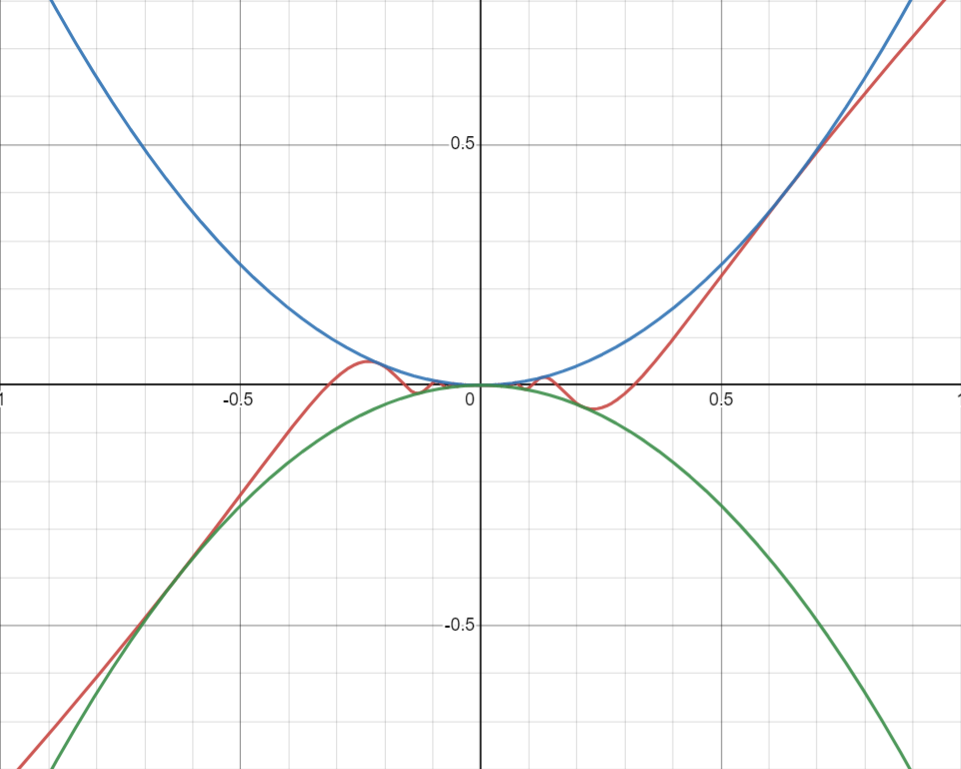
\includegraphics[width=0.4\linewidth]{E:/UBC/Year-3/Term-1/MATH 320/Notes/Images/1.png}
	\caption{Plot of \(y=x^2\sin{\left(\displaystyle\frac{1}{x}\right)}\) from desmos; the red curve is \(y\).}
\end{figure}

\begin{figure}[H]
	\centering
	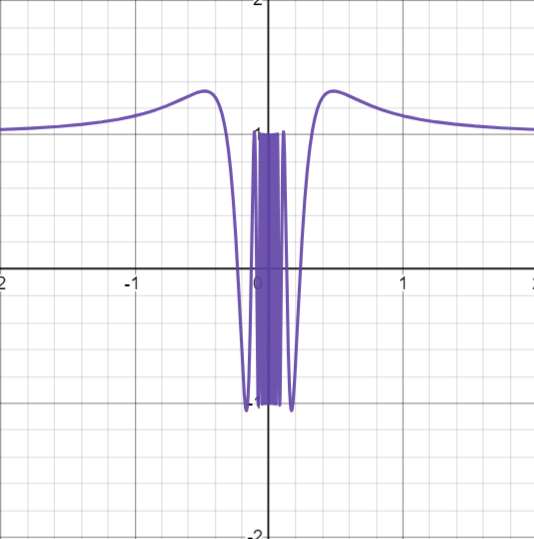
\includegraphics[width=0.4\linewidth]{E:/UBC/Year-3/Term-1/MATH 320/Notes/Images/2.png}
	\caption{Plot of \(y=f'(x)\) from Desmos.}
\end{figure}